
	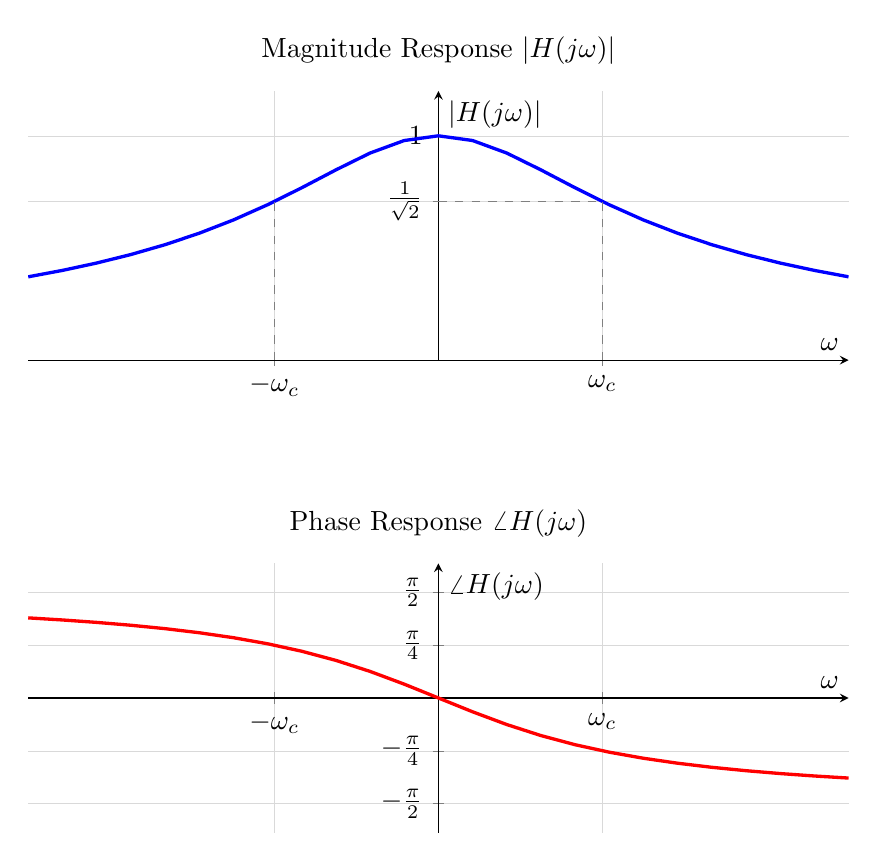
\begin{tikzpicture}
		% Define a common style
		\pgfplotsset{
			lpf a/.style={
				width=12cm, height=5cm,
				axis lines=middle, xlabel={$\omega$},
				xmin=-5, xmax=5,
				xtick={-2, 2},
				grid=major, grid style={line width=.1pt, draw=gray!30},
				no marks,
			}
		}
		
		% Top plot: Magnitude
		\begin{scope}[yshift=6cm]
			\begin{axis}[
				lpf a,
				title={Magnitude Response $|H(j\omega)|$},
				ylabel={$|H(j\omega)|$},
				ymin=0, ymax=1.2,
				xticklabels={$-\omega_c$, $\omega_c$},
				ytick={0.707, 1},
				yticklabels={$\frac{1}{\sqrt{2}}$, $1$},
				]
				\addplot[blue, very thick, domain=-5:5] {1 / sqrt(1 + (x/2)^2)};
				\draw[dashed, gray] (axis cs:2,0) -- (axis cs:2, {1/sqrt(2)});
				\draw[dashed, gray] (axis cs:-2,0) -- (axis cs:-2, {1/sqrt(2)});
				\draw[dashed, gray] (axis cs:0,{1/sqrt(2)}) -- (axis cs:2, {1/sqrt(2)});
			\end{axis}
		\end{scope}
		
		% Bottom plot: Phase
		\begin{scope}[yshift=0cm]
			\begin{axis}[
				lpf a,
				title={Phase Response $\angle H(j\omega)$},
				ylabel={$\angle H(j\omega)$},
				ymin=-2, ymax=2,
				xticklabels={$-\omega_c$, $\omega_c$},
				ytick={-1.57, -0.785, 0.785, 1.57},
				yticklabels={$-\frac{\pi}{2}$, $-\frac{\pi}{4}$, $\frac{\pi}{4}$, $\frac{\pi}{2}$},
				]
				% --- FIXED LINE ---
				% Convert atan output (degrees) to radians by multiplying by pi/180
				\addplot[red, very thick, domain=-5:5] {-atan(x/2) * pi/180};
			\end{axis}
		\end{scope}
	\end{tikzpicture}
	








